\documentclass{beamer}

\usepackage{siunitx}
\usepackage{graphicx}

\usetheme{Montpellier}

\title{Effect of low-rise building geometry on tornado-induced loads}
\author{140926~WANG Yong}
\institute{Southeast University}
\date{\today}

\begin{document}

\begin{frame}
	\titlepage
\end{frame}

\section*{Outline}
\begin{frame}
	\tableofcontents
\end{frame}

\section{Introduction}

\begin{frame}
    \frametitle{Challenges to quantify  tornado-induced loads:}
    \begin{itemize}
    	\item<1-> Lack of research facilities capable of determining tornado-induced loads (pressures, forces, etc.)
    	\item<2-> Absence of full-scale data
    	\item<3-> Lack of interest in tornado-resistant design
    \end{itemize}
\end{frame}

\begin{frame}
    \frametitle{How to overcome these challenges:}
    \begin{itemize}
    	\item<1-> Iowa State University (ISU) tornado simulator
    	\item<2-> Full-scale data from several recent tornados
    	\item<3-> Pressures obtained form  the ISU simulator are verified
    \end{itemize}
\end{frame}


\section{Description of simulated tornado}
\subsection{Maximum horizonal wind speed}

\begin{frame}
	\frametitle{Maximum horizontal wind speed}
	\begin{description}
		\item[Fact 1:  ]<1-> Around 90\% of all tornados are rated F2 or less
		\item[Fact 2: ]<2-> Maximum velocity of F2 tornado is \alert{\SI{74}{m/s}}
		\item[Fact 3: ]<3-> Design wind speed ranges from \alert{\SI{63}{m/s}} to \alert{\SI{80}{m/s}} (ASCE 7-10, 2010)
		\item[Fact 4: ]<4-> Maximum horizonal velocity of the tornado generated by ISU Simulator is \alert{\SI{11.7}{m/s}}
	\end{description}
	\begin{block}<5->{Choose target full-scale wind speed to be \alert{\SI{74}{m/s}}}
			 Velocity scale $\lambda_v=11.7/74=1/6.3$
	\end{block} 
\end{frame}

\begin{frame}
	\frametitle{Contour plot of normalized tangential velocity}
	\begin{figure}
	\centering
	\caption{Contour plot of tangential velocity magnitudes normalized with respect to the maximum tangential velocity}
	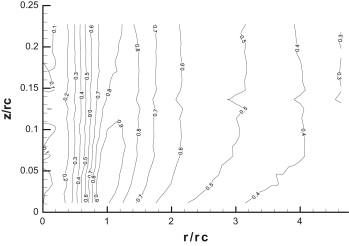
\includegraphics{./fig/1.jpg}
	\end{figure}

\end{frame}

\subsection{Tornado vortex diameter}

\begin{frame}
	\frametitle{Tornado vortex diameter}
	\begin{definition}
	 	\alert{Radius of the core $r_c$}: radius of the maximum wind near the ground
	\end{definition}
	\begin{description}
		\item[Fact 1: ]<2-> $r_c$ of F2 tornado is between \alert{\SI{45}{} to \SI{225}{m}}
		\item[Fact 2: ]<3-> $r_c$ of simulated tornado is \alert{\SI{0.56}{m}}
	\end{description}
	\begin{block}<4->{Choose $r_c$ of target full-scale tornado to be \alert{\SI{56}{m}}}
		   Length scale is $1:100$ 
	\end{block} 
\end{frame}

\subsection{Swirl ratio}

\begin{frame}
	\frametitle{Swirl ratio: definition}
	\begin{definition}
		\alert{Swirl ratio $S$}: 
		$$ S = \frac{\pi V_{\theta\mathrm{max}} r_c^2}{Q}$$
		\begin{description}
			\item[$r_c$: ] core radius
			\item[$V_{\theta\mathrm{max}}$: ] maximum tangential wind speed
			\item[$Q$: ] inflow rate of the vortex measured at $r=r_c$
		\end{description}
	\end{definition}
\end{frame}

\begin{frame}
	\frametitle{How to choose swirl ratio}
		\begin{description}
			\item[Fact 1: ] <2-> Data from full-scale tornados indicates \alert{$S\geqslant2.0$}
			\item[Fact 2: ]<3-> Best fit of full-scale data with numerical simulation when \alert{$S\geqslant2.0$}
		\end{description}
		\begin{block}<4->{Choose the swirl ratio $S$  to be \alert{\num{2.6}} }
			
		\end{block}
\end{frame}


\section{Model description, instruments,  conventions}
\subsection{Building models}
\begin{frame}
	\frametitle{Building models}
	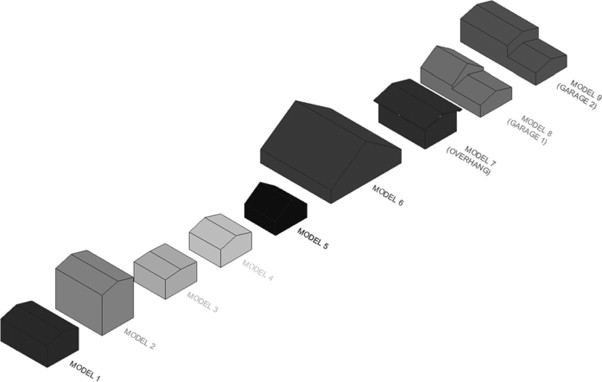
\includegraphics[width=0.8\textwidth]{./fig/2.jpg}
\end{frame}
\begin{frame}
	\frametitle{Model dimensions}
	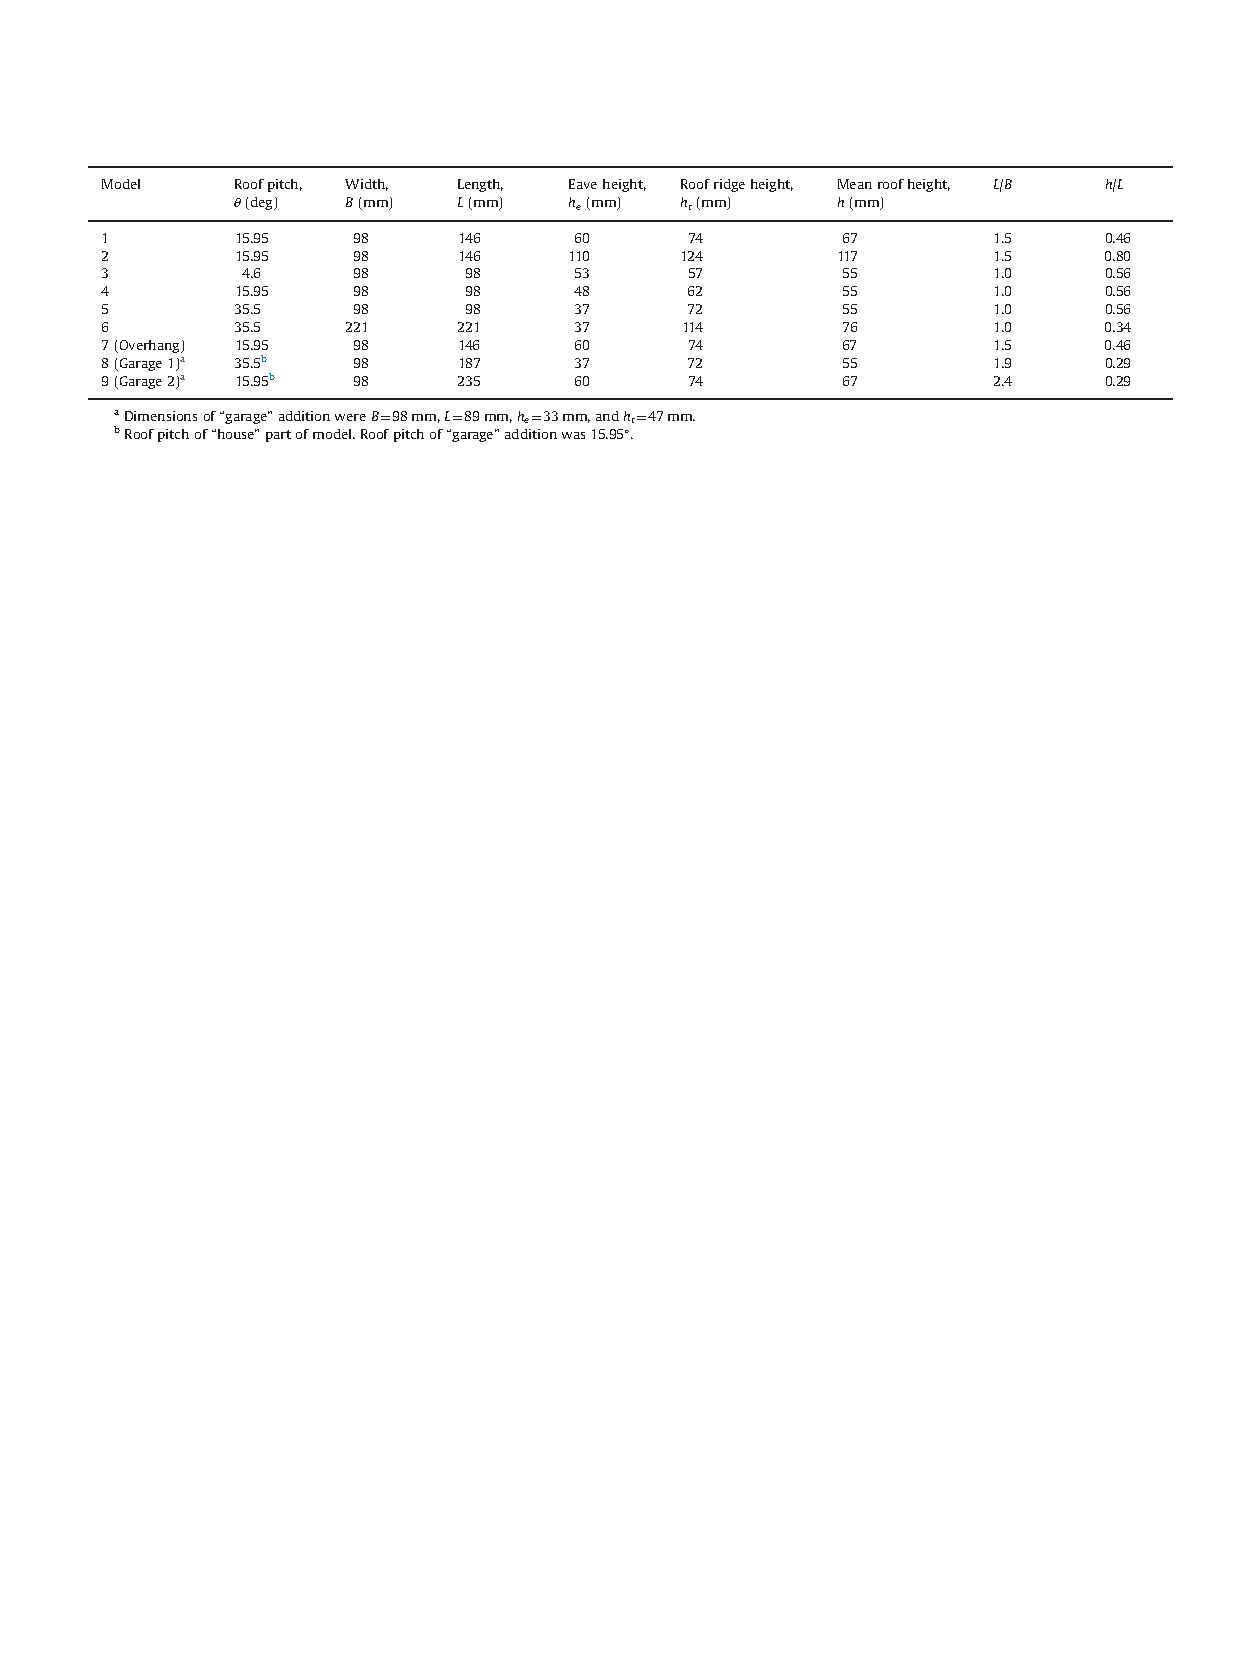
\includegraphics[width=\textwidth]{./fig/model_dimension.pdf}
\end{frame}

\subsection{Instrumentation}
\begin{frame}
	\frametitle{Wind velocity measurement: Cobra probe}
	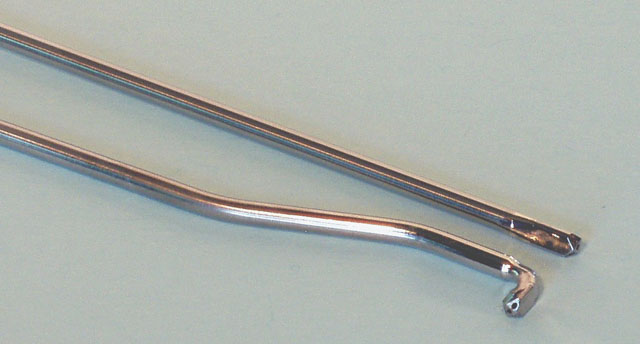
\includegraphics[width=0.6\textwidth]{./fig/speed_measure.jpg}
	\begin{block}<2->{Measurement points}
	horizontally spaced at \SI{50.8}{mm}
	
	vertically spaced at \SI{6.35}{mm}
	\end{block}
\end{frame}
\begin{frame}
	\frametitle{Pressure measurement: ZOC33/64Px pressure transducer}
	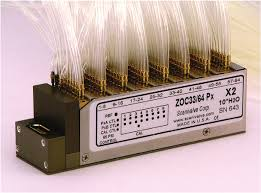
\includegraphics[width=0.6\textwidth]{./fig/pressure_measure.jpg}
		\begin{block}<2->{Measurement frequency: \SI{390}{Hz}}
		
		\end{block}
\end{frame}

\subsection{Procedure and conventions}
\begin{frame}
	\frametitle{Procedure}
	\begin{itemize}
		\item<1-> For each test case the pressure were recorded 10 times
		\item<2-> Calculate the peak pressure as the average of the peak pressures from each of the 10 runs
		\item<3> Change the BOA from \ang{0} to \ang{90} with a step size of \ang{15}
	\end{itemize}
	\begin{definition}<3>
		\alert{BOA}: the orientation of the building with respect to the direction of translation of the tornado
	\end{definition}
\end{frame}

\begin{frame}
	\frametitle{BOA \& Areas used to compute force coefficients}
	\begin{figure}
	\centering
	\caption{Building orientation angle (BOA) with respect to the tornado translation axis (X) and areas ($S_v$, $S_z$) used to normalize force coefficients}
		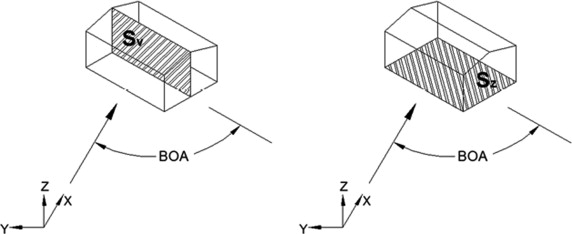
\includegraphics[width=\textwidth]{./fig/3.jpg}
	\end{figure}
	
	
\end{frame}

\begin{frame}
	\frametitle{Calculation of force coefficients}
	\begin{equation}
		C_{Fx}=\frac{F_x}{(1/2)\rho V_H^2 S_v}
	\end{equation}
	
	\begin{equation}
		C_{Fy}=\frac{F_y}{(1/2)\rho V_H^2 S_v}
	\end{equation}
	
	\begin{equation}
		C_{Fz}=\frac{F_z}{(1/2)\rho V_H^2 S_z}
	\end{equation}
	
	\begin{equation}
		C_{Fxy}=\sqrt{C_{Fx}^2+C_{Fy}^2}
	\end{equation}
\end{frame}

\section{Results}
\subsection{The effect of cave height}
\begin{frame}
	\frametitle{The effect of eave height: Models}
	\begin{description}
		\item[Fact 1: ]<1-> Difference between Model 1 \& 2 was \alert{eave heights $h_e$}
		\item[Fact 2: ]<2-> Model 1:  $h_e=\SI{110}{mm}$ \\
		                                         Model 2:  $h_e=\SI{60}{mm}$
	\end{description}
\end{frame}
\begin{frame}
	\frametitle{The effect of eave height: Peak pressures}
	\begin{figure}
		\centering
		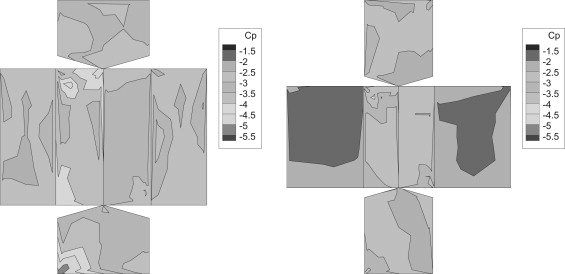
\includegraphics[width=0.8\textwidth]{./fig/4.jpg}
		\caption{Peak pressure contours for Model 1 (left) \& 2 (right), BOA=\ang{30}}
	\end{figure}
	\begin{itemize}
		\item Peak pressure contours of Model 1 \& 2 are similar
		\item Magnitudes of peak pressure: Model 1 $>$ Model 2
	\end{itemize}
\end{frame}

\begin{frame}
	\frametitle{The effect of eave height: Vertical force coefficient}
	\begin{figure}
		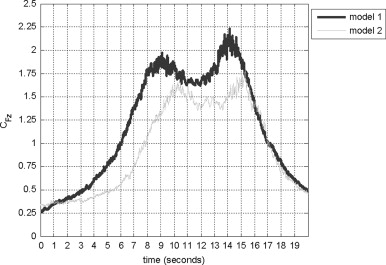
\includegraphics[width=0.8\textwidth]{./fig/5.jpg}
		\caption{$C_{Fz}$ time history for Model 1 \& 2, BOA=\ang{30}}
	\end{figure}
\end{frame}

\begin{frame}
	\frametitle{The effect of eave height: XY force coefficient}
	\begin{figure}
			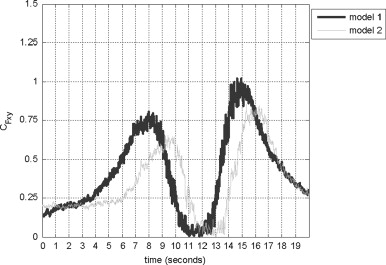
\includegraphics[width=0.8\textwidth]{./fig/6.jpg}
			\caption{$C_{Fxy}$ time history for Models 1 \& 2, BOA=\ang{30}}
		\end{figure}
\end{frame}

\subsection{The effect of roof pitch}
\begin{frame}
	\frametitle{The effect of roof pitch: Models}
	\begin{description}
		\item[Fact 1: ]<1-> Difference between Model 3, 4  \& 5 was \alert{roof pitch $\theta$}
		\item[Fact 2: ]<2-> Model 3:  $\theta=\ang{4.6}$ \\
		                                         Model 4:  $\theta=\ang{15.95}$ \\
		                                         Model 5:  $\theta=\ang{35.5}$
	\end{description}
\end{frame}

\begin{frame}
	\frametitle{The effect of roof pitch: Peak pressures}
	\begin{figure}
		\centering
		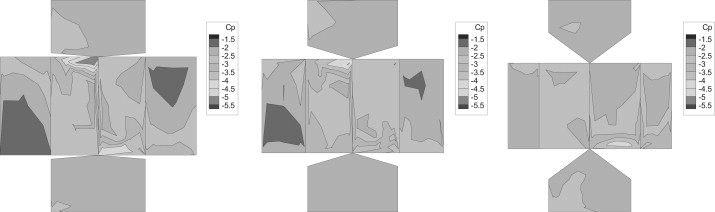
\includegraphics[width=\textwidth]{./fig/7.jpg}
		\caption{Peak pressure contours for Model 3 (left), 4 (center) \& 5 (right), BOA=\ang{45}}
	\end{figure}
	\begin{itemize}
		\item As $\theta$ $\uparrow$, peak pressure magnitudes for the \alert{roof} $\downarrow$
		\item As $\theta$ $\uparrow$, peak pressure magnitudes for the \alert{wall} $\uparrow$
	\end{itemize}
\end{frame}

\begin{frame}
	\frametitle{The effect of roof pitch: Vertical force coefficient}
	\begin{figure}
		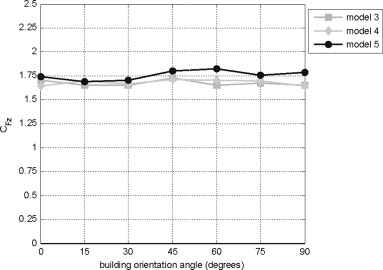
\includegraphics[width=0.8\textwidth]{./fig/8.jpg}
		\caption{$C_{Fz}$ time history for Models 3, 4 \& 5, for each BOA}
	\end{figure}
\end{frame}

\begin{frame}
	\frametitle{The effect of roof pitch: Vertical force coefficient}
	\begin{figure}
			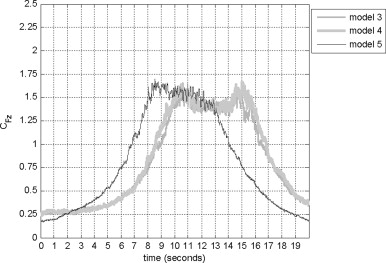
\includegraphics[width=0.8\textwidth]{./fig/9.jpg}
			\caption{$C_{Fz}$ time history for Models 3, 4 \& 5, BOA=\ang{30}}
		\end{figure}
\end{frame}


\section*{The End}
\begin{frame}
\begin{figure}
\centering

\includegraphics[width=\textwidth]{./fig/thank_you.jpg}
\end{figure}

\end{frame}

\end{document}